\documentclass[1p]{elsarticle_modified}
%\bibliographystyle{elsarticle-num}

%\usepackage[colorlinks]{hyperref}
%\usepackage{abbrmath_seonhwa} %\Abb, \Ascr, \Acal ,\Abf, \Afrak
\usepackage{amsfonts}
\usepackage{amssymb}
\usepackage{amsmath}
\usepackage{amsthm}
\usepackage{scalefnt}
\usepackage{amsbsy}
\usepackage{kotex}
\usepackage{caption}
\usepackage{subfig}
\usepackage{color}
\usepackage{graphicx}
\usepackage{xcolor} %% white, black, red, green, blue, cyan, magenta, yellow
\usepackage{float}
\usepackage{setspace}
\usepackage{hyperref}

\usepackage{tikz}
\usetikzlibrary{arrows}

\usepackage{multirow}
\usepackage{array} % fixed length table
\usepackage{hhline}

%%%%%%%%%%%%%%%%%%%%%
\makeatletter
\renewcommand*\env@matrix[1][\arraystretch]{%
	\edef\arraystretch{#1}%
	\hskip -\arraycolsep
	\let\@ifnextchar\new@ifnextchar
	\array{*\c@MaxMatrixCols c}}
\makeatother %https://tex.stackexchange.com/questions/14071/how-can-i-increase-the-line-spacing-in-a-matrix
%%%%%%%%%%%%%%%

\usepackage[normalem]{ulem}

\newcommand{\msout}[1]{\ifmmode\text{\sout{\ensuremath{#1}}}\else\sout{#1}\fi}
%SOURCE: \msout is \stkout macro in https://tex.stackexchange.com/questions/20609/strikeout-in-math-mode

\newcommand{\cancel}[1]{
	\ifmmode
	{\color{red}\msout{#1}}
	\else
	{\color{red}\sout{#1}}
	\fi
}

\newcommand{\add}[1]{
	{\color{blue}\uwave{#1}}
}

\newcommand{\replace}[2]{
	\ifmmode
	{\color{red}\msout{#1}}{\color{blue}\uwave{#2}}
	\else
	{\color{red}\sout{#1}}{\color{blue}\uwave{#2}}
	\fi
}

\newcommand{\Sol}{\mathcal{S}} %segment
\newcommand{\D}{D} %diagram
\newcommand{\A}{\mathcal{A}} %arc


%%%%%%%%%%%%%%%%%%%%%%%%%%%%%5 test

\def\sl{\operatorname{\textup{SL}}(2,\Cbb)}
\def\psl{\operatorname{\textup{PSL}}(2,\Cbb)}
\def\quan{\mkern 1mu \triangleright \mkern 1mu}

\theoremstyle{definition}
\newtheorem{thm}{Theorem}[section]
\newtheorem{prop}[thm]{Proposition}
\newtheorem{lem}[thm]{Lemma}
\newtheorem{ques}[thm]{Question}
\newtheorem{cor}[thm]{Corollary}
\newtheorem{defn}[thm]{Definition}
\newtheorem{exam}[thm]{Example}
\newtheorem{rmk}[thm]{Remark}
\newtheorem{alg}[thm]{Algorithm}

\newcommand{\I}{\sqrt{-1}}
\begin{document}

%\begin{frontmatter}
%
%\title{Boundary parabolic representations of knots up to 8 crossings}
%
%%% Group authors per affiliation:
%\author{Yunhi Cho} 
%\address{Department of Mathematics, University of Seoul, Seoul, Korea}
%\ead{yhcho@uos.ac.kr}
%
%
%\author{Seonhwa Kim} %\fnref{s_kim}}
%\address{Center for Geometry and Physics, Institute for Basic Science, Pohang, 37673, Korea}
%\ead{ryeona17@ibs.re.kr}
%
%\author{Hyuk Kim}
%\address{Department of Mathematical Sciences, Seoul National University, Seoul 08826, Korea}
%\ead{hyukkim@snu.ac.kr}
%
%\author{Seokbeom Yoon}
%\address{Department of Mathematical Sciences, Seoul National University, Seoul, 08826,  Korea}
%\ead{sbyoon15@snu.ac.kr}
%
%\begin{abstract}
%We find all boundary parabolic representation of knots up to 8 crossings.
%
%\end{abstract}
%\begin{keyword}
%    \MSC[2010] 57M25 
%\end{keyword}
%
%\end{frontmatter}

%\linenumbers
%\tableofcontents
%
\newcommand\colored[1]{\textcolor{white}{\rule[-0.35ex]{0.8em}{1.4ex}}\kern-0.8em\color{red} #1}%
%\newcommand\colored[1]{\textcolor{white}{ #1}\kern-2.17ex	\textcolor{white}{ #1}\kern-1.81ex	\textcolor{white}{ #1}\kern-2.15ex\color{red}#1	}

{\Large $\underline{12a_{0553}~(K12a_{0553})}$}

\setlength{\tabcolsep}{10pt}
\renewcommand{\arraystretch}{1.6}
\vspace{1cm}\begin{tabular}{m{100pt}>{\centering\arraybackslash}m{274pt}}
\multirow{5}{120pt}{
	\centering
	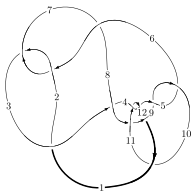
\includegraphics[width=112pt]{../../../GIT/diagram.site/Diagrams/png/1354_12a_0553.png}\\
\ \ \ A knot diagram\footnotemark}&
\allowdisplaybreaks
\textbf{Linearized knot diagam} \\
\cline{2-2}
 &
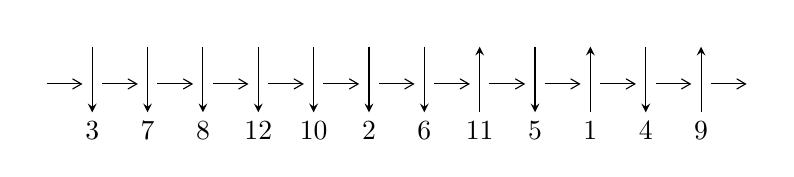
\begin{tikzpicture}[x=20pt, y=17pt]
	% nodes
	\node (C0) at (0, 0) {};
	\node (C1) at (1, 0) {};
	\node (C1U) at (1, +1) {};
	\node (C1D) at (1, -1) {3};

	\node (C2) at (2, 0) {};
	\node (C2U) at (2, +1) {};
	\node (C2D) at (2, -1) {7};

	\node (C3) at (3, 0) {};
	\node (C3U) at (3, +1) {};
	\node (C3D) at (3, -1) {8};

	\node (C4) at (4, 0) {};
	\node (C4U) at (4, +1) {};
	\node (C4D) at (4, -1) {12};

	\node (C5) at (5, 0) {};
	\node (C5U) at (5, +1) {};
	\node (C5D) at (5, -1) {10};

	\node (C6) at (6, 0) {};
	\node (C6U) at (6, +1) {};
	\node (C6D) at (6, -1) {2};

	\node (C7) at (7, 0) {};
	\node (C7U) at (7, +1) {};
	\node (C7D) at (7, -1) {6};

	\node (C8) at (8, 0) {};
	\node (C8U) at (8, +1) {};
	\node (C8D) at (8, -1) {11};

	\node (C9) at (9, 0) {};
	\node (C9U) at (9, +1) {};
	\node (C9D) at (9, -1) {5};

	\node (C10) at (10, 0) {};
	\node (C10U) at (10, +1) {};
	\node (C10D) at (10, -1) {1};

	\node (C11) at (11, 0) {};
	\node (C11U) at (11, +1) {};
	\node (C11D) at (11, -1) {4};

	\node (C12) at (12, 0) {};
	\node (C12U) at (12, +1) {};
	\node (C12D) at (12, -1) {9};
	\node (C13) at (13, 0) {};

	% arrows
	\draw[->,>={angle 60}]
	(C0) edge (C1) (C1) edge (C2) (C2) edge (C3) (C3) edge (C4) (C4) edge (C5) (C5) edge (C6) (C6) edge (C7) (C7) edge (C8) (C8) edge (C9) (C9) edge (C10) (C10) edge (C11) (C11) edge (C12) (C12) edge (C13) ;	\draw[->,>=stealth]
	(C1U) edge (C1D) (C2U) edge (C2D) (C3U) edge (C3D) (C4U) edge (C4D) (C5U) edge (C5D) (C6U) edge (C6D) (C7U) edge (C7D) (C8D) edge (C8U) (C9U) edge (C9D) (C10D) edge (C10U) (C11U) edge (C11D) (C12D) edge (C12U) ;
	\end{tikzpicture} \\
\hhline{~~} \\& 
\textbf{Solving Sequence} \\ \cline{2-2} 
 &
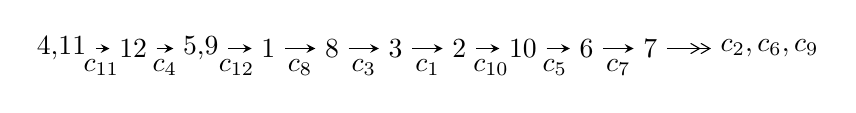
\begin{tikzpicture}[x=23pt, y=7pt]
	% node
	\node (A0) at (-1/8, 0) {4,11};
	\node (A1) at (1, 0) {12};
	\node (A2) at (33/16, 0) {5,9};
	\node (A3) at (25/8, 0) {1};
	\node (A4) at (33/8, 0) {8};
	\node (A5) at (41/8, 0) {3};
	\node (A6) at (49/8, 0) {2};
	\node (A7) at (57/8, 0) {10};
	\node (A8) at (65/8, 0) {6};
	\node (A9) at (73/8, 0) {7};
	\node (C1) at (1/2, -1) {$c_{11}$};
	\node (C2) at (3/2, -1) {$c_{4}$};
	\node (C3) at (21/8, -1) {$c_{12}$};
	\node (C4) at (29/8, -1) {$c_{8}$};
	\node (C5) at (37/8, -1) {$c_{3}$};
	\node (C6) at (45/8, -1) {$c_{1}$};
	\node (C7) at (53/8, -1) {$c_{10}$};
	\node (C8) at (61/8, -1) {$c_{5}$};
	\node (C9) at (69/8, -1) {$c_{7}$};
	\node (A10) at (11, 0) {$c_{2},c_{6},c_{9}$};

	% edge
	\draw[->,>=stealth]	
	(A0) edge (A1) (A1) edge (A2) (A2) edge (A3) (A3) edge (A4) (A4) edge (A5) (A5) edge (A6) (A6) edge (A7) (A7) edge (A8) (A8) edge (A9) ;
	\draw[->>,>={angle 60}]	
	(A9) edge (A10);
\end{tikzpicture} \\ 

\end{tabular} \\

\footnotetext{
The image of knot diagram is generated by the software ``\textbf{Draw programme}" developed by Andrew Bartholomew(\url{http://www.layer8.co.uk/maths/draw/index.htm\#Running-draw}), where we modified some parts for our purpose(\url{https://github.com/CATsTAILs/LinksPainter}).
}\phantom \\ \newline 
\centering \textbf{Ideals for irreducible components\footnotemark of $X_{\text{par}}$} 
 
\begin{align*}
I^u_{1}&=\langle 
2.25623\times10^{23} u^{41}+9.66993\times10^{22} u^{40}+\cdots+3.04045\times10^{23} b+5.01776\times10^{23},\\
\phantom{I^u_{1}}&\phantom{= \langle  }-4.05453\times10^{23} u^{41}-3.26106\times10^{23} u^{40}+\cdots+3.04045\times10^{23} a-8.85169\times10^{23},\;u^{42}+u^{41}+\cdots+5 u+1\rangle \\
I^u_{2}&=\langle 
-1.69030\times10^{239} u^{79}+4.53403\times10^{239} u^{78}+\cdots+5.27838\times10^{239} b+3.07543\times10^{239},\\
\phantom{I^u_{2}}&\phantom{= \langle  }4.23498\times10^{239} u^{79}-1.43076\times10^{239} u^{78}+\cdots+5.27838\times10^{239} a+5.44531\times10^{240},\;u^{80}- u^{79}+\cdots+16 u+1\rangle \\
I^u_{3}&=\langle 
u^2+b-1,\;u^{19}+u^{18}+\cdots+a+2,\;u^{20}+u^{19}+\cdots+6 u-1\rangle \\
\\
\end{align*}
\raggedright * 3 irreducible components of $\dim_{\mathbb{C}}=0$, with total 142 representations.\\
\footnotetext{All coefficients of polynomials are rational numbers. But the coefficients are sometimes approximated in decimal forms when there is not enough margin.}
\newpage
\renewcommand{\arraystretch}{1}
\centering \section*{I. $I^u_{1}= \langle 2.26\times10^{23} u^{41}+9.67\times10^{22} u^{40}+\cdots+3.04\times10^{23} b+5.02\times10^{23},\;-4.05\times10^{23} u^{41}-3.26\times10^{23} u^{40}+\cdots+3.04\times10^{23} a-8.85\times10^{23},\;u^{42}+u^{41}+\cdots+5 u+1 \rangle$}
\flushleft \textbf{(i) Arc colorings}\\
\begin{tabular}{m{7pt} m{180pt} m{7pt} m{180pt} }
\flushright $a_{4}=$&$\begin{pmatrix}0\\u\end{pmatrix}$ \\
\flushright $a_{11}=$&$\begin{pmatrix}1\\0\end{pmatrix}$ \\
\flushright $a_{12}=$&$\begin{pmatrix}1\\u^2\end{pmatrix}$ \\
\flushright $a_{5}=$&$\begin{pmatrix}- u\\- u^3+u\end{pmatrix}$ \\
\flushright $a_{9}=$&$\begin{pmatrix}1.33353 u^{41}+1.07256 u^{40}+\cdots+5.15836 u+2.91131\\-0.742070 u^{41}-0.318043 u^{40}+\cdots-5.18702 u-1.65034\end{pmatrix}$ \\
\flushright $a_{1}=$&$\begin{pmatrix}-0.356219 u^{41}-0.656913 u^{40}+\cdots+1.83103 u+1.56167\\0.742070 u^{41}+0.318043 u^{40}+\cdots+5.18702 u+1.65034\end{pmatrix}$ \\
\flushright $a_{8}=$&$\begin{pmatrix}2.07560 u^{41}+1.39060 u^{40}+\cdots+10.3454 u+4.56165\\-0.742070 u^{41}-0.318043 u^{40}+\cdots-5.18702 u-1.65034\end{pmatrix}$ \\
\flushright $a_{3}=$&$\begin{pmatrix}-0.137641 u^{41}-0.218884 u^{40}+\cdots+0.646429 u-0.235243\\-0.424027 u^{41}-0.699003 u^{40}+\cdots-1.06001 u-0.742070\end{pmatrix}$ \\
\flushright $a_{2}=$&$\begin{pmatrix}0.682566 u^{41}+0.629255 u^{40}+\cdots+0.728245 u+1.43319\\1.27131 u^{41}+1.19520 u^{40}+\cdots+4.41786 u+1.76416\end{pmatrix}$ \\
\flushright $a_{10}=$&$\begin{pmatrix}1.33353 u^{41}+1.07256 u^{40}+\cdots+5.15836 u+2.91131\\-0.742070 u^{41}-0.318043 u^{40}+\cdots-5.18702 u-1.65034\end{pmatrix}$ \\
\flushright $a_{6}=$&$\begin{pmatrix}0.260974 u^{41}-0.330487 u^{40}+\cdots+2.75635 u+1.33353\\-0.424027 u^{41}-0.699003 u^{40}+\cdots-1.06001 u-0.742070\end{pmatrix}$ \\
\flushright $a_{7}=$&$\begin{pmatrix}1.01423 u^{41}-0.256599 u^{40}+\cdots+12.9428 u+5.13247\\-1.27131 u^{41}-1.19520 u^{40}+\cdots-4.41786 u-1.76416\end{pmatrix}$\\&\end{tabular}
\flushleft \textbf{(ii) Obstruction class $= -1$}\\~\\
\flushleft \textbf{(iii) Cusp Shapes $= \frac{758348575428048311643999}{304044864012407159949563} u^{41}-\frac{189703780989871384844127}{304044864012407159949563} u^{40}+\cdots-\frac{773024156845572154682826}{304044864012407159949563} u-\frac{2397936412798830570628702}{304044864012407159949563}$}\\~\\
\newpage\renewcommand{\arraystretch}{1}
\flushleft \textbf{(iv) u-Polynomials at the component}\newline \\
\begin{tabular}{m{50pt}|m{274pt}}
Crossings & \hspace{64pt}u-Polynomials at each crossing \\
\hline $$\begin{aligned}c_{1},c_{7}\end{aligned}$$&$\begin{aligned}
&u^{42}+14 u^{41}+\cdots+92 u+16
\end{aligned}$\\
\hline $$\begin{aligned}c_{2},c_{6}\end{aligned}$$&$\begin{aligned}
&u^{42}-6 u^{41}+\cdots+26 u-4
\end{aligned}$\\
\hline $$\begin{aligned}c_{3}\end{aligned}$$&$\begin{aligned}
&u^{42}+6 u^{41}+\cdots-97086 u-58612
\end{aligned}$\\
\hline $$\begin{aligned}c_{4},c_{5},c_{9}\\c_{11}\end{aligned}$$&$\begin{aligned}
&u^{42}+u^{41}+\cdots+5 u+1
\end{aligned}$\\
\hline $$\begin{aligned}c_{8},c_{10}\end{aligned}$$&$\begin{aligned}
&u^{42}-3 u^{41}+\cdots-4 u-1
\end{aligned}$\\
\hline $$\begin{aligned}c_{12}\end{aligned}$$&$\begin{aligned}
&u^{42}-44 u^{41}+\cdots+18874368 u-1048576
\end{aligned}$\\
\hline
\end{tabular}\\~\\
\newpage\renewcommand{\arraystretch}{1}
\flushleft \textbf{(v) Riley Polynomials at the component}\newline \\
\begin{tabular}{m{50pt}|m{274pt}}
Crossings & \hspace{64pt}Riley Polynomials at each crossing \\
\hline $$\begin{aligned}c_{1},c_{7}\end{aligned}$$&$\begin{aligned}
&y^{42}+26 y^{41}+\cdots+10512 y+256
\end{aligned}$\\
\hline $$\begin{aligned}c_{2},c_{6}\end{aligned}$$&$\begin{aligned}
&y^{42}-14 y^{41}+\cdots-92 y+16
\end{aligned}$\\
\hline $$\begin{aligned}c_{3}\end{aligned}$$&$\begin{aligned}
&y^{42}-22 y^{41}+\cdots-37177652828 y+3435366544
\end{aligned}$\\
\hline $$\begin{aligned}c_{4},c_{5},c_{9}\\c_{11}\end{aligned}$$&$\begin{aligned}
&y^{42}-33 y^{41}+\cdots-5 y+1
\end{aligned}$\\
\hline $$\begin{aligned}c_{8},c_{10}\end{aligned}$$&$\begin{aligned}
&y^{42}+5 y^{41}+\cdots-102 y+1
\end{aligned}$\\
\hline $$\begin{aligned}c_{12}\end{aligned}$$&$\begin{aligned}
&y^{42}+4 y^{41}+\cdots-24739011624960 y+1099511627776
\end{aligned}$\\
\hline
\end{tabular}\\~\\
\newpage\flushleft \textbf{(vi) Complex Volumes and Cusp Shapes}
$$\begin{array}{c|c|c}  
\text{Solutions to }I^u_{1}& \I (\text{vol} + \sqrt{-1}CS) & \text{Cusp shape}\\
 \hline 
\begin{aligned}
u &= -0.129110 + 0.837718 I \\
a &= \phantom{-}0.208797 + 0.545010 I \\
b &= \phantom{-}0.766049 - 0.963564 I\end{aligned}
 & \phantom{-}1.83605 - 7.68678 I & -3.96818 + 6.98985 I \\ \hline\begin{aligned}
u &= -0.129110 - 0.837718 I \\
a &= \phantom{-}0.208797 - 0.545010 I \\
b &= \phantom{-}0.766049 + 0.963564 I\end{aligned}
 & \phantom{-}1.83605 + 7.68678 I & -3.96818 - 6.98985 I \\ \hline\begin{aligned}
u &= -1.183880 + 0.049134 I \\
a &= -1.11857 + 1.10941 I \\
b &= \phantom{-}0.682568 + 0.572973 I\end{aligned}
 & -3.35379 + 2.88258 I & -9.71297 - 5.70027 I \\ \hline\begin{aligned}
u &= -1.183880 - 0.049134 I \\
a &= -1.11857 - 1.10941 I \\
b &= \phantom{-}0.682568 - 0.572973 I\end{aligned}
 & -3.35379 - 2.88258 I & -9.71297 + 5.70027 I \\ \hline\begin{aligned}
u &= -1.186440 + 0.119570 I \\
a &= -0.77152 - 2.13314 I \\
b &= \phantom{-}0.091296 - 0.620171 I\end{aligned}
 & -5.41447 + 1.52315 I & -20.8164 - 2.3413 I \\ \hline\begin{aligned}
u &= -1.186440 - 0.119570 I \\
a &= -0.77152 + 2.13314 I \\
b &= \phantom{-}0.091296 + 0.620171 I\end{aligned}
 & -5.41447 - 1.52315 I & -20.8164 + 2.3413 I \\ \hline\begin{aligned}
u &= \phantom{-}0.154286 + 0.788847 I \\
a &= \phantom{-}0.196401 - 0.509540 I \\
b &= \phantom{-}0.810088 + 0.862295 I\end{aligned}
 & \phantom{-}2.84163 + 2.23994 I & -1.58112 - 1.75265 I \\ \hline\begin{aligned}
u &= \phantom{-}0.154286 - 0.788847 I \\
a &= \phantom{-}0.196401 + 0.509540 I \\
b &= \phantom{-}0.810088 - 0.862295 I\end{aligned}
 & \phantom{-}2.84163 - 2.23994 I & -1.58112 + 1.75265 I \\ \hline\begin{aligned}
u &= -1.130060 + 0.426134 I \\
a &= \phantom{-}0.34478 - 1.74706 I \\
b &= -0.649711 - 0.498795 I\end{aligned}
 & \phantom{-}0.35921 + 3.98317 I & -5.18876 - 5.91925 I \\ \hline\begin{aligned}
u &= -1.130060 - 0.426134 I \\
a &= \phantom{-}0.34478 + 1.74706 I \\
b &= -0.649711 + 0.498795 I\end{aligned}
 & \phantom{-}0.35921 - 3.98317 I & -5.18876 + 5.91925 I\\
 \hline 
 \end{array}$$\newpage$$\begin{array}{c|c|c}  
\text{Solutions to }I^u_{1}& \I (\text{vol} + \sqrt{-1}CS) & \text{Cusp shape}\\
 \hline 
\begin{aligned}
u &= \phantom{-}1.213330 + 0.075694 I \\
a &= -0.94606 - 1.09355 I \\
b &= \phantom{-}0.759589 - 0.683845 I\end{aligned}
 & -4.83918 - 8.81290 I & -11.6564 + 8.5892 I \\ \hline\begin{aligned}
u &= \phantom{-}1.213330 - 0.075694 I \\
a &= -0.94606 + 1.09355 I \\
b &= \phantom{-}0.759589 + 0.683845 I\end{aligned}
 & -4.83918 + 8.81290 I & -11.6564 - 8.5892 I \\ \hline\begin{aligned}
u &= \phantom{-}0.005260 + 0.776538 I \\
a &= \phantom{-}0.315859 + 0.529708 I \\
b &= \phantom{-}0.489355 - 0.846533 I\end{aligned}
 & -2.63776 - 2.01463 I & -9.50411 + 3.62154 I \\ \hline\begin{aligned}
u &= \phantom{-}0.005260 - 0.776538 I \\
a &= \phantom{-}0.315859 - 0.529708 I \\
b &= \phantom{-}0.489355 + 0.846533 I\end{aligned}
 & -2.63776 + 2.01463 I & -9.50411 - 3.62154 I \\ \hline\begin{aligned}
u &= \phantom{-}0.215406 + 0.717843 I \\
a &= \phantom{-}0.498976 + 0.594478 I \\
b &= \phantom{-}0.083209 - 0.718916 I\end{aligned}
 & \phantom{-}1.03284 + 3.43933 I & -5.25606 - 1.29339 I \\ \hline\begin{aligned}
u &= \phantom{-}0.215406 - 0.717843 I \\
a &= \phantom{-}0.498976 - 0.594478 I \\
b &= \phantom{-}0.083209 + 0.718916 I\end{aligned}
 & \phantom{-}1.03284 - 3.43933 I & -5.25606 + 1.29339 I \\ \hline\begin{aligned}
u &= \phantom{-}1.250870 + 0.029270 I \\
a &= -0.86186 + 1.52627 I \\
b &= \phantom{-}0.402311 + 0.797420 I\end{aligned}
 & -10.43820 + 1.64027 I & -19.3366 - 4.1061 I \\ \hline\begin{aligned}
u &= \phantom{-}1.250870 - 0.029270 I \\
a &= -0.86186 - 1.52627 I \\
b &= \phantom{-}0.402311 - 0.797420 I\end{aligned}
 & -10.43820 - 1.64027 I & -19.3366 + 4.1061 I \\ \hline\begin{aligned}
u &= \phantom{-}1.183600 + 0.466397 I \\
a &= \phantom{-}0.26597 + 1.64501 I \\
b &= -0.767402 + 0.595298 I\end{aligned}
 & -0.04073 - 10.00640 I & -6.00000 + 9.99752 I \\ \hline\begin{aligned}
u &= \phantom{-}1.183600 - 0.466397 I \\
a &= \phantom{-}0.26597 - 1.64501 I \\
b &= -0.767402 - 0.595298 I\end{aligned}
 & -0.04073 + 10.00640 I & -6.00000 - 9.99752 I\\
 \hline 
 \end{array}$$\newpage$$\begin{array}{c|c|c}  
\text{Solutions to }I^u_{1}& \I (\text{vol} + \sqrt{-1}CS) & \text{Cusp shape}\\
 \hline 
\begin{aligned}
u &= \phantom{-}1.275990 + 0.184603 I \\
a &= -0.37506 + 1.80775 I \\
b &= -0.074450 + 0.897247 I\end{aligned}
 & -8.35329 - 6.18961 I & -17.4347 + 7.3045 I \\ \hline\begin{aligned}
u &= \phantom{-}1.275990 - 0.184603 I \\
a &= -0.37506 - 1.80775 I \\
b &= -0.074450 - 0.897247 I\end{aligned}
 & -8.35329 + 6.18961 I & -17.4347 - 7.3045 I \\ \hline\begin{aligned}
u &= -0.540941 + 0.438454 I \\
a &= -0.141478 + 0.341563 I \\
b &= \phantom{-}1.289300 - 0.240168 I\end{aligned}
 & \phantom{-}4.31778 + 3.64803 I & -4.57023 - 8.96524 I \\ \hline\begin{aligned}
u &= -0.540941 - 0.438454 I \\
a &= -0.141478 - 0.341563 I \\
b &= \phantom{-}1.289300 + 0.240168 I\end{aligned}
 & \phantom{-}4.31778 - 3.64803 I & -4.57023 + 8.96524 I \\ \hline\begin{aligned}
u &= \phantom{-}0.468364 + 0.499939 I \\
a &= -0.071909 - 0.357763 I \\
b &= \phantom{-}1.241650 + 0.335026 I\end{aligned}
 & \phantom{-}4.66986 + 1.75891 I & -1.95443 + 2.74065 I \\ \hline\begin{aligned}
u &= \phantom{-}0.468364 - 0.499939 I \\
a &= -0.071909 + 0.357763 I \\
b &= \phantom{-}1.241650 - 0.335026 I\end{aligned}
 & \phantom{-}4.66986 - 1.75891 I & -1.95443 - 2.74065 I \\ \hline\begin{aligned}
u &= -0.267732 + 0.602998 I \\
a &= \phantom{-}0.630356 - 0.557804 I \\
b &= \phantom{-}0.005521 + 0.517110 I\end{aligned}
 & \phantom{-}1.74525 + 1.74697 I & -3.78653 - 4.83256 I \\ \hline\begin{aligned}
u &= -0.267732 - 0.602998 I \\
a &= \phantom{-}0.630356 + 0.557804 I \\
b &= \phantom{-}0.005521 - 0.517110 I\end{aligned}
 & \phantom{-}1.74525 - 1.74697 I & -3.78653 + 4.83256 I \\ \hline\begin{aligned}
u &= \phantom{-}0.088989 + 0.553108 I \\
a &= \phantom{-}0.258260 - 0.292992 I \\
b &= \phantom{-}0.693618 + 0.405730 I\end{aligned}
 & \phantom{-}1.27279 + 1.01412 I & \phantom{-}1.95077 - 3.41118 I \\ \hline\begin{aligned}
u &= \phantom{-}0.088989 - 0.553108 I \\
a &= \phantom{-}0.258260 + 0.292992 I \\
b &= \phantom{-}0.693618 - 0.405730 I\end{aligned}
 & \phantom{-}1.27279 - 1.01412 I & \phantom{-}1.95077 + 3.41118 I\\
 \hline 
 \end{array}$$\newpage$$\begin{array}{c|c|c}  
\text{Solutions to }I^u_{1}& \I (\text{vol} + \sqrt{-1}CS) & \text{Cusp shape}\\
 \hline 
\begin{aligned}
u &= \phantom{-}1.42369 + 0.44997 I \\
a &= \phantom{-}0.01185 + 1.47417 I \\
b &= -0.87902 + 1.23053 I\end{aligned}
 & -7.37891 - 9.51051 I & \phantom{-0.000000 } 0 \\ \hline\begin{aligned}
u &= \phantom{-}1.42369 - 0.44997 I \\
a &= \phantom{-}0.01185 - 1.47417 I \\
b &= -0.87902 - 1.23053 I\end{aligned}
 & -7.37891 + 9.51051 I & \phantom{-0.000000 } 0 \\ \hline\begin{aligned}
u &= -1.44107 + 0.39945 I \\
a &= -0.03941 - 1.48174 I \\
b &= -0.74204 - 1.31355 I\end{aligned}
 & -9.51277 + 4.75387 I & \phantom{-0.000000 } 0 \\ \hline\begin{aligned}
u &= -1.44107 - 0.39945 I \\
a &= -0.03941 + 1.48174 I \\
b &= -0.74204 + 1.31355 I\end{aligned}
 & -9.51277 - 4.75387 I & \phantom{-0.000000 } 0 \\ \hline\begin{aligned}
u &= -0.467313\phantom{ +0.000000I} \\
a &= -0.190127\phantom{ +0.000000I} \\
b &= \phantom{-}1.14861\phantom{ +0.000000I}\end{aligned}
 & \phantom{-}0.327792\phantom{ +0.000000I} & -22.7930\phantom{ +0.000000I} \\ \hline\begin{aligned}
u &= -1.47914 + 0.46825 I \\
a &= \phantom{-}0.00076 - 1.42482 I \\
b &= -0.97294 - 1.38112 I\end{aligned}
 & -12.2925 + 11.8405 I & \phantom{-0.000000 } 0 \\ \hline\begin{aligned}
u &= -1.47914 - 0.46825 I \\
a &= \phantom{-}0.00076 + 1.42482 I \\
b &= -0.97294 + 1.38112 I\end{aligned}
 & -12.2925 - 11.8405 I & \phantom{-0.000000 } 0 \\ \hline\begin{aligned}
u &= \phantom{-}1.46466 + 0.51916 I \\
a &= \phantom{-}0.039566 + 1.412300 I \\
b &= -1.11314 + 1.29694 I\end{aligned}
 & -5.76180 - 12.68780 I & \phantom{-0.000000 } 0 \\ \hline\begin{aligned}
u &= \phantom{-}1.46466 - 0.51916 I \\
a &= \phantom{-}0.039566 - 1.412300 I \\
b &= -1.11314 - 1.29694 I\end{aligned}
 & -5.76180 + 12.68780 I & \phantom{-0.000000 } 0 \\ \hline\begin{aligned}
u &= -1.48417 + 0.52390 I \\
a &= \phantom{-}0.033655 - 1.398890 I \\
b &= -1.14418 - 1.35093 I\end{aligned}
 & -7.0633 + 18.4553 I & \phantom{-0.000000 } 0\\
 \hline 
 \end{array}$$\newpage$$\begin{array}{c|c|c}  
\text{Solutions to }I^u_{1}& \I (\text{vol} + \sqrt{-1}CS) & \text{Cusp shape}\\
 \hline 
\begin{aligned}
u &= -1.48417 - 0.52390 I \\
a &= \phantom{-}0.033655 + 1.398890 I \\
b &= -1.14418 + 1.35093 I\end{aligned}
 & -7.0633 - 18.4553 I & \phantom{-0.000000 } 0 \\ \hline\begin{aligned}
u &= -0.336499\phantom{ +0.000000I} \\
a &= \phantom{-}1.23139\phantom{ +0.000000I} \\
b &= -0.0919546\phantom{ +0.000000I}\end{aligned}
 & -0.740467\phantom{ +0.000000I} & -14.2860\phantom{ +0.000000I}\\
 \hline 
 \end{array}$$\newpage\newpage\renewcommand{\arraystretch}{1}
\centering \section*{II. $I^u_{2}= \langle -1.69\times10^{239} u^{79}+4.53\times10^{239} u^{78}+\cdots+5.28\times10^{239} b+3.08\times10^{239},\;4.23\times10^{239} u^{79}-1.43\times10^{239} u^{78}+\cdots+5.28\times10^{239} a+5.45\times10^{240},\;u^{80}- u^{79}+\cdots+16 u+1 \rangle$}
\flushleft \textbf{(i) Arc colorings}\\
\begin{tabular}{m{7pt} m{180pt} m{7pt} m{180pt} }
\flushright $a_{4}=$&$\begin{pmatrix}0\\u\end{pmatrix}$ \\
\flushright $a_{11}=$&$\begin{pmatrix}1\\0\end{pmatrix}$ \\
\flushright $a_{12}=$&$\begin{pmatrix}1\\u^2\end{pmatrix}$ \\
\flushright $a_{5}=$&$\begin{pmatrix}- u\\- u^3+u\end{pmatrix}$ \\
\flushright $a_{9}=$&$\begin{pmatrix}-0.802325 u^{79}+0.271060 u^{78}+\cdots-1089.56 u-10.3162\\0.320231 u^{79}-0.858981 u^{78}+\cdots-20.8795 u-0.582647\end{pmatrix}$ \\
\flushright $a_{1}=$&$\begin{pmatrix}-0.516068 u^{79}+0.487109 u^{78}+\cdots-516.254 u+26.4919\\-0.202847 u^{79}+0.477995 u^{78}+\cdots-29.2026 u-0.0849526\end{pmatrix}$ \\
\flushright $a_{8}=$&$\begin{pmatrix}-1.12256 u^{79}+1.13004 u^{78}+\cdots-1068.68 u-9.73360\\0.320231 u^{79}-0.858981 u^{78}+\cdots-20.8795 u-0.582647\end{pmatrix}$ \\
\flushright $a_{3}=$&$\begin{pmatrix}-1.80579 u^{79}+1.76789 u^{78}+\cdots-1294.87 u-2.86959\\-0.636707 u^{79}+1.41921 u^{78}+\cdots-39.0595 u-1.05782\end{pmatrix}$ \\
\flushright $a_{2}=$&$\begin{pmatrix}0.876128 u^{79}-0.791821 u^{78}+\cdots+867.674 u+19.7324\\0.852252 u^{79}-1.81244 u^{78}+\cdots+21.8245 u+1.25344\end{pmatrix}$ \\
\flushright $a_{10}=$&$\begin{pmatrix}-1.03160 u^{79}+0.833907 u^{78}+\cdots-1094.09 u-10.5337\\0.161944 u^{79}-0.475631 u^{78}+\cdots-21.4547 u-0.698779\end{pmatrix}$ \\
\flushright $a_{6}=$&$\begin{pmatrix}1.94294 u^{79}-2.11379 u^{78}+\cdots+1397.76 u+4.71417\\-0.448779 u^{79}+0.963456 u^{78}+\cdots+30.0345 u+0.437105\end{pmatrix}$ \\
\flushright $a_{7}=$&$\begin{pmatrix}0.731095 u^{79}-0.879762 u^{78}+\cdots+444.056 u-14.4550\\-0.724590 u^{79}+1.48433 u^{78}+\cdots+9.28280 u-0.670444\end{pmatrix}$\\&\end{tabular}
\flushleft \textbf{(ii) Obstruction class $= -1$}\\~\\
\flushleft \textbf{(iii) Cusp Shapes $= -1.89162 u^{79}+4.42072 u^{78}+\cdots-12.3040 u-15.1389$}\\~\\
\newpage\renewcommand{\arraystretch}{1}
\flushleft \textbf{(iv) u-Polynomials at the component}\newline \\
\begin{tabular}{m{50pt}|m{274pt}}
Crossings & \hspace{64pt}u-Polynomials at each crossing \\
\hline $$\begin{aligned}c_{1},c_{7}\end{aligned}$$&$\begin{aligned}
&(u^{20}+7 u^{19}+\cdots+6 u+1)^{4}
\end{aligned}$\\
\hline $$\begin{aligned}c_{2},c_{6}\end{aligned}$$&$\begin{aligned}
&(u^{20}+u^{19}+\cdots+3 u^2-1)^{4}
\end{aligned}$\\
\hline $$\begin{aligned}c_{3}\end{aligned}$$&$\begin{aligned}
&(u^{20}- u^{19}+\cdots+4 u-1)^{4}
\end{aligned}$\\
\hline $$\begin{aligned}c_{4},c_{5},c_{9}\\c_{11}\end{aligned}$$&$\begin{aligned}
&u^{80}- u^{79}+\cdots+16 u+1
\end{aligned}$\\
\hline $$\begin{aligned}c_{8},c_{10}\end{aligned}$$&$\begin{aligned}
&u^{80}+23 u^{79}+\cdots+798776 u+37537
\end{aligned}$\\
\hline $$\begin{aligned}c_{12}\end{aligned}$$&$\begin{aligned}
&(u^2+u+1)^{40}
\end{aligned}$\\
\hline
\end{tabular}\\~\\
\newpage\renewcommand{\arraystretch}{1}
\flushleft \textbf{(v) Riley Polynomials at the component}\newline \\
\begin{tabular}{m{50pt}|m{274pt}}
Crossings & \hspace{64pt}Riley Polynomials at each crossing \\
\hline $$\begin{aligned}c_{1},c_{7}\end{aligned}$$&$\begin{aligned}
&(y^{20}+13 y^{19}+\cdots-6 y+1)^{4}
\end{aligned}$\\
\hline $$\begin{aligned}c_{2},c_{6}\end{aligned}$$&$\begin{aligned}
&(y^{20}-7 y^{19}+\cdots-6 y+1)^{4}
\end{aligned}$\\
\hline $$\begin{aligned}c_{3}\end{aligned}$$&$\begin{aligned}
&(y^{20}-11 y^{19}+\cdots-6 y+1)^{4}
\end{aligned}$\\
\hline $$\begin{aligned}c_{4},c_{5},c_{9}\\c_{11}\end{aligned}$$&$\begin{aligned}
&y^{80}-69 y^{79}+\cdots+1440 y+1
\end{aligned}$\\
\hline $$\begin{aligned}c_{8},c_{10}\end{aligned}$$&$\begin{aligned}
&y^{80}+27 y^{79}+\cdots+9352736088 y+1409026369
\end{aligned}$\\
\hline $$\begin{aligned}c_{12}\end{aligned}$$&$\begin{aligned}
&(y^2+y+1)^{40}
\end{aligned}$\\
\hline
\end{tabular}\\~\\
\newpage\flushleft \textbf{(vi) Complex Volumes and Cusp Shapes}
$$\begin{array}{c|c|c}  
\text{Solutions to }I^u_{2}& \I (\text{vol} + \sqrt{-1}CS) & \text{Cusp shape}\\
 \hline 
\begin{aligned}
u &= \phantom{-}0.207784 + 0.987527 I \\
a &= \phantom{-}0.445184 - 0.154793 I \\
b &= -0.851402 - 0.539056 I\end{aligned}
 & \phantom{-}3.03993 + 4.87637 I & \phantom{-0.000000 } 0 \\ \hline\begin{aligned}
u &= \phantom{-}0.207784 - 0.987527 I \\
a &= \phantom{-}0.445184 + 0.154793 I \\
b &= -0.851402 + 0.539056 I\end{aligned}
 & \phantom{-}3.03993 - 4.87637 I & \phantom{-0.000000 } 0 \\ \hline\begin{aligned}
u &= -0.951078 + 0.228099 I \\
a &= \phantom{-}0.55710 + 1.83713 I \\
b &= \phantom{-}0.772031 + 0.458447 I\end{aligned}
 & \phantom{-}3.03993 - 0.81660 I & \phantom{-0.000000 } 0 \\ \hline\begin{aligned}
u &= -0.951078 - 0.228099 I \\
a &= \phantom{-}0.55710 - 1.83713 I \\
b &= \phantom{-}0.772031 - 0.458447 I\end{aligned}
 & \phantom{-}3.03993 + 0.81660 I & \phantom{-0.000000 } 0 \\ \hline\begin{aligned}
u &= \phantom{-}0.996696 + 0.266242 I \\
a &= \phantom{-}0.44755 - 1.84281 I \\
b &= \phantom{-}0.890900 - 0.596478 I\end{aligned}
 & \phantom{-}3.03993 - 4.87637 I & \phantom{-0.000000 } 0 \\ \hline\begin{aligned}
u &= \phantom{-}0.996696 - 0.266242 I \\
a &= \phantom{-}0.44755 + 1.84281 I \\
b &= \phantom{-}0.890900 + 0.596478 I\end{aligned}
 & \phantom{-}3.03993 + 4.87637 I & \phantom{-0.000000 } 0 \\ \hline\begin{aligned}
u &= -0.275813 + 0.910568 I \\
a &= \phantom{-}0.560339 + 0.160187 I \\
b &= -0.841509 + 0.463941 I\end{aligned}
 & \phantom{-}3.03993 + 0.81660 I & \phantom{-0.000000 } 0 \\ \hline\begin{aligned}
u &= -0.275813 - 0.910568 I \\
a &= \phantom{-}0.560339 - 0.160187 I \\
b &= -0.841509 - 0.463941 I\end{aligned}
 & \phantom{-}3.03993 - 0.81660 I & \phantom{-0.000000 } 0 \\ \hline\begin{aligned}
u &= -0.240644 + 1.064020 I \\
a &= \phantom{-}0.010895 - 0.165200 I \\
b &= -0.596302 - 0.694141 I\end{aligned}
 & -2.17062 + 4.19124 I & \phantom{-0.000000 } 0 \\ \hline\begin{aligned}
u &= -0.240644 - 1.064020 I \\
a &= \phantom{-}0.010895 + 0.165200 I \\
b &= -0.596302 + 0.694141 I\end{aligned}
 & -2.17062 - 4.19124 I & \phantom{-0.000000 } 0\\
 \hline 
 \end{array}$$\newpage$$\begin{array}{c|c|c}  
\text{Solutions to }I^u_{2}& \I (\text{vol} + \sqrt{-1}CS) & \text{Cusp shape}\\
 \hline 
\begin{aligned}
u &= -0.899552 + 0.699001 I \\
a &= -0.555723 + 0.260013 I \\
b &= -0.351175 - 0.083803 I\end{aligned}
 & -3.26827 + 4.38821 I & \phantom{-0.000000 } 0 \\ \hline\begin{aligned}
u &= -0.899552 - 0.699001 I \\
a &= -0.555723 - 0.260013 I \\
b &= -0.351175 + 0.083803 I\end{aligned}
 & -3.26827 - 4.38821 I & \phantom{-0.000000 } 0 \\ \hline\begin{aligned}
u &= \phantom{-}0.518571 + 1.015560 I \\
a &= -0.211103 + 0.058336 I \\
b &= -0.400489 + 0.599197 I\end{aligned}
 & -3.66592 + 0.10467 I & \phantom{-0.000000 } 0 \\ \hline\begin{aligned}
u &= \phantom{-}0.518571 - 1.015560 I \\
a &= -0.211103 - 0.058336 I \\
b &= -0.400489 - 0.599197 I\end{aligned}
 & -3.66592 - 0.10467 I & \phantom{-0.000000 } 0 \\ \hline\begin{aligned}
u &= -1.140030 + 0.123562 I \\
a &= \phantom{-}0.558917 - 1.144130 I \\
b &= -0.104456 - 0.760969 I\end{aligned}
 & -2.17062 + 0.13148 I & \phantom{-0.000000 } 0 \\ \hline\begin{aligned}
u &= -1.140030 - 0.123562 I \\
a &= \phantom{-}0.558917 + 1.144130 I \\
b &= -0.104456 + 0.760969 I\end{aligned}
 & -2.17062 - 0.13148 I & \phantom{-0.000000 } 0 \\ \hline\begin{aligned}
u &= \phantom{-}0.788041 + 0.320938 I \\
a &= -1.165290 - 0.395640 I \\
b &= -0.903502 + 0.071649 I\end{aligned}
 & -3.26827 + 0.32844 I & \phantom{-0.000000 } 0 \\ \hline\begin{aligned}
u &= \phantom{-}0.788041 - 0.320938 I \\
a &= -1.165290 + 0.395640 I \\
b &= -0.903502 - 0.071649 I\end{aligned}
 & -3.26827 - 0.32844 I & \phantom{-0.000000 } 0 \\ \hline\begin{aligned}
u &= \phantom{-}1.180310 + 0.012052 I \\
a &= -0.91234 - 1.30364 I \\
b &= -1.73380 - 0.97589 I\end{aligned}
 & -5.25931 - 1.21416 I & \phantom{-0.000000 } 0 \\ \hline\begin{aligned}
u &= \phantom{-}1.180310 - 0.012052 I \\
a &= -0.91234 + 1.30364 I \\
b &= -1.73380 + 0.97589 I\end{aligned}
 & -5.25931 + 1.21416 I & \phantom{-0.000000 } 0\\
 \hline 
 \end{array}$$\newpage$$\begin{array}{c|c|c}  
\text{Solutions to }I^u_{2}& \I (\text{vol} + \sqrt{-1}CS) & \text{Cusp shape}\\
 \hline 
\begin{aligned}
u &= -1.111090 + 0.442655 I \\
a &= \phantom{-}0.654258 - 0.784229 I \\
b &= -0.591917 - 0.592017 I\end{aligned}
 & -0.50419 + 2.40320 I & \phantom{-0.000000 } 0 \\ \hline\begin{aligned}
u &= -1.111090 - 0.442655 I \\
a &= \phantom{-}0.654258 + 0.784229 I \\
b &= -0.591917 + 0.592017 I\end{aligned}
 & -0.50419 - 2.40320 I & \phantom{-0.000000 } 0 \\ \hline\begin{aligned}
u &= -1.198430 + 0.027915 I \\
a &= -0.92147 - 1.37061 I \\
b &= -1.91445 - 1.03978 I\end{aligned}
 & -6.41764 + 4.04252 I & \phantom{-0.000000 } 0 \\ \hline\begin{aligned}
u &= -1.198430 - 0.027915 I \\
a &= -0.92147 + 1.37061 I \\
b &= -1.91445 + 1.03978 I\end{aligned}
 & -6.41764 - 4.04252 I & \phantom{-0.000000 } 0 \\ \hline\begin{aligned}
u &= \phantom{-}1.224920 + 0.184610 I \\
a &= -0.680597 - 1.092490 I \\
b &= -1.00390 - 1.04377 I\end{aligned}
 & -5.61498 - 2.02988 I & \phantom{-0.000000 } 0 \\ \hline\begin{aligned}
u &= \phantom{-}1.224920 - 0.184610 I \\
a &= -0.680597 + 1.092490 I \\
b &= -1.00390 + 1.04377 I\end{aligned}
 & -5.61498 + 2.02988 I & \phantom{-0.000000 } 0 \\ \hline\begin{aligned}
u &= \phantom{-}1.214950 + 0.272262 I \\
a &= \phantom{-}0.12453 - 1.65766 I \\
b &= \phantom{-}0.77124 - 1.37558 I\end{aligned}
 & -2.17062 - 4.19124 I & \phantom{-0.000000 } 0 \\ \hline\begin{aligned}
u &= \phantom{-}1.214950 - 0.272262 I \\
a &= \phantom{-}0.12453 + 1.65766 I \\
b &= \phantom{-}0.77124 + 1.37558 I\end{aligned}
 & -2.17062 + 4.19124 I & \phantom{-0.000000 } 0 \\ \hline\begin{aligned}
u &= -1.269020 + 0.005894 I \\
a &= -0.80674 + 1.39166 I \\
b &= -1.77834 + 1.38715 I\end{aligned}
 & -10.49270 + 2.02988 I & \phantom{-0.000000 } 0 \\ \hline\begin{aligned}
u &= -1.269020 - 0.005894 I \\
a &= -0.80674 - 1.39166 I \\
b &= -1.77834 - 1.38715 I\end{aligned}
 & -10.49270 - 2.02988 I & \phantom{-0.000000 } 0\\
 \hline 
 \end{array}$$\newpage$$\begin{array}{c|c|c}  
\text{Solutions to }I^u_{2}& \I (\text{vol} + \sqrt{-1}CS) & \text{Cusp shape}\\
 \hline 
\begin{aligned}
u &= \phantom{-}1.176100 + 0.483198 I \\
a &= \phantom{-}0.592616 + 0.752617 I \\
b &= -0.674058 + 0.672840 I\end{aligned}
 & -1.65238 - 8.02785 I & \phantom{-0.000000 } 0 \\ \hline\begin{aligned}
u &= \phantom{-}1.176100 - 0.483198 I \\
a &= \phantom{-}0.592616 - 0.752617 I \\
b &= -0.674058 - 0.672840 I\end{aligned}
 & -1.65238 + 8.02785 I & \phantom{-0.000000 } 0 \\ \hline\begin{aligned}
u &= \phantom{-}1.221650 + 0.370872 I \\
a &= \phantom{-}0.05476 - 1.79734 I \\
b &= \phantom{-}1.20285 - 1.51952 I\end{aligned}
 & -0.50419 - 6.46297 I & \phantom{-0.000000 } 0 \\ \hline\begin{aligned}
u &= \phantom{-}1.221650 - 0.370872 I \\
a &= \phantom{-}0.05476 + 1.79734 I \\
b &= \phantom{-}1.20285 + 1.51952 I\end{aligned}
 & -0.50419 + 6.46297 I & \phantom{-0.000000 } 0 \\ \hline\begin{aligned}
u &= \phantom{-}0.340631 + 1.244900 I \\
a &= -0.0068353 + 0.0139151 I \\
b &= -0.502001 + 0.840278 I\end{aligned}
 & -6.59138 - 5.99841 I & \phantom{-0.000000 } 0 \\ \hline\begin{aligned}
u &= \phantom{-}0.340631 - 1.244900 I \\
a &= -0.0068353 - 0.0139151 I \\
b &= -0.502001 - 0.840278 I\end{aligned}
 & -6.59138 + 5.99841 I & \phantom{-0.000000 } 0 \\ \hline\begin{aligned}
u &= -1.239340 + 0.384198 I \\
a &= \phantom{-}0.02492 + 1.80581 I \\
b &= \phantom{-}1.25428 + 1.61735 I\end{aligned}
 & -1.65238 + 12.08760 I & \phantom{-0.000000 } 0 \\ \hline\begin{aligned}
u &= -1.239340 - 0.384198 I \\
a &= \phantom{-}0.02492 - 1.80581 I \\
b &= \phantom{-}1.25428 - 1.61735 I\end{aligned}
 & -1.65238 - 12.08760 I & \phantom{-0.000000 } 0 \\ \hline\begin{aligned}
u &= \phantom{-}1.262130 + 0.312419 I \\
a &= \phantom{-}0.500943 + 0.892680 I \\
b &= -0.454901 + 0.863903 I\end{aligned}
 & -6.59138 - 1.93864 I & \phantom{-0.000000 } 0 \\ \hline\begin{aligned}
u &= \phantom{-}1.262130 - 0.312419 I \\
a &= \phantom{-}0.500943 - 0.892680 I \\
b &= -0.454901 - 0.863903 I\end{aligned}
 & -6.59138 + 1.93864 I & \phantom{-0.000000 } 0\\
 \hline 
 \end{array}$$\newpage$$\begin{array}{c|c|c}  
\text{Solutions to }I^u_{2}& \I (\text{vol} + \sqrt{-1}CS) & \text{Cusp shape}\\
 \hline 
\begin{aligned}
u &= -1.268080 + 0.331222 I \\
a &= \phantom{-}0.00849 + 1.71936 I \\
b &= \phantom{-}0.95703 + 1.70298 I\end{aligned}
 & -6.59138 + 5.99841 I & \phantom{-0.000000 } 0 \\ \hline\begin{aligned}
u &= -1.268080 - 0.331222 I \\
a &= \phantom{-}0.00849 - 1.71936 I \\
b &= \phantom{-}0.95703 - 1.70298 I\end{aligned}
 & -6.59138 - 5.99841 I & \phantom{-0.000000 } 0 \\ \hline\begin{aligned}
u &= \phantom{-}1.314510 + 0.067425 I \\
a &= -0.68640 - 1.37199 I \\
b &= -1.43973 - 1.62011 I\end{aligned}
 & -5.25931 - 2.84561 I & \phantom{-0.000000 } 0 \\ \hline\begin{aligned}
u &= \phantom{-}1.314510 - 0.067425 I \\
a &= -0.68640 + 1.37199 I \\
b &= -1.43973 + 1.62011 I\end{aligned}
 & -5.25931 + 2.84561 I & \phantom{-0.000000 } 0 \\ \hline\begin{aligned}
u &= -0.198524 + 1.302860 I \\
a &= \phantom{-}0.0821657 - 0.0079703 I \\
b &= -0.640357 - 0.895315 I\end{aligned}
 & -0.50419 + 6.46297 I & \phantom{-0.000000 } 0 \\ \hline\begin{aligned}
u &= -0.198524 - 1.302860 I \\
a &= \phantom{-}0.0821657 + 0.0079703 I \\
b &= -0.640357 + 0.895315 I\end{aligned}
 & -0.50419 - 6.46297 I & \phantom{-0.000000 } 0 \\ \hline\begin{aligned}
u &= -1.329160 + 0.038165 I \\
a &= -0.70698 + 1.42142 I \\
b &= -1.60376 + 1.71482 I\end{aligned}
 & -6.41764 + 8.10228 I & \phantom{-0.000000 } 0 \\ \hline\begin{aligned}
u &= -1.329160 - 0.038165 I \\
a &= -0.70698 - 1.42142 I \\
b &= -1.60376 - 1.71482 I\end{aligned}
 & -6.41764 - 8.10228 I & \phantom{-0.000000 } 0 \\ \hline\begin{aligned}
u &= -1.307500 + 0.242820 I \\
a &= -0.02283 + 1.54565 I \\
b &= \phantom{-}0.44377 + 1.69971 I\end{aligned}
 & -3.66592 - 0.10467 I & \phantom{-0.000000 } 0 \\ \hline\begin{aligned}
u &= -1.307500 - 0.242820 I \\
a &= -0.02283 - 1.54565 I \\
b &= \phantom{-}0.44377 - 1.69971 I\end{aligned}
 & -3.66592 + 0.10467 I & \phantom{-0.000000 } 0\\
 \hline 
 \end{array}$$\newpage$$\begin{array}{c|c|c}  
\text{Solutions to }I^u_{2}& \I (\text{vol} + \sqrt{-1}CS) & \text{Cusp shape}\\
 \hline 
\begin{aligned}
u &= \phantom{-}0.227721 + 1.347240 I \\
a &= \phantom{-}0.0715746 - 0.0185276 I \\
b &= -0.614831 + 0.942610 I\end{aligned}
 & -1.65238 - 12.08760 I & \phantom{-0.000000 } 0 \\ \hline\begin{aligned}
u &= \phantom{-}0.227721 - 1.347240 I \\
a &= \phantom{-}0.0715746 + 0.0185276 I \\
b &= -0.614831 - 0.942610 I\end{aligned}
 & -1.65238 + 12.08760 I & \phantom{-0.000000 } 0 \\ \hline\begin{aligned}
u &= \phantom{-}1.366970 + 0.076347 I \\
a &= \phantom{-}0.287797 + 1.039200 I \\
b &= -0.180804 + 1.129850 I\end{aligned}
 & -3.66592 + 4.16444 I & \phantom{-0.000000 } 0 \\ \hline\begin{aligned}
u &= \phantom{-}1.366970 - 0.076347 I \\
a &= \phantom{-}0.287797 - 1.039200 I \\
b &= -0.180804 - 1.129850 I\end{aligned}
 & -3.66592 - 4.16444 I & \phantom{-0.000000 } 0 \\ \hline\begin{aligned}
u &= \phantom{-}1.373280 + 0.192811 I \\
a &= -0.212459 - 1.275000 I \\
b &= -0.21758 - 1.60360 I\end{aligned}
 & -3.26827 - 4.38821 I & \phantom{-0.000000 } 0 \\ \hline\begin{aligned}
u &= \phantom{-}1.373280 - 0.192811 I \\
a &= -0.212459 + 1.275000 I \\
b &= -0.21758 + 1.60360 I\end{aligned}
 & -3.26827 + 4.38821 I & \phantom{-0.000000 } 0 \\ \hline\begin{aligned}
u &= -1.46328 + 0.16377 I \\
a &= -0.056126 + 1.023110 I \\
b &= -0.128306 + 1.324110 I\end{aligned}
 & -3.26827 - 0.32844 I & \phantom{-0.000000 } 0 \\ \hline\begin{aligned}
u &= -1.46328 - 0.16377 I \\
a &= -0.056126 - 1.023110 I \\
b &= -0.128306 - 1.324110 I\end{aligned}
 & -3.26827 + 0.32844 I & \phantom{-0.000000 } 0 \\ \hline\begin{aligned}
u &= -1.40433 + 0.49536 I \\
a &= -0.316968 + 0.709311 I \\
b &= -0.060476 + 0.799784 I\end{aligned}
 & -5.61498 + 2.02988 I & \phantom{-0.000000 } 0 \\ \hline\begin{aligned}
u &= -1.40433 - 0.49536 I \\
a &= -0.316968 - 0.709311 I \\
b &= -0.060476 - 0.799784 I\end{aligned}
 & -5.61498 - 2.02988 I & \phantom{-0.000000 } 0\\
 \hline 
 \end{array}$$\newpage$$\begin{array}{c|c|c}  
\text{Solutions to }I^u_{2}& \I (\text{vol} + \sqrt{-1}CS) & \text{Cusp shape}\\
 \hline 
\begin{aligned}
u &= -0.303297 + 0.220517 I \\
a &= -2.32870 - 1.44235 I \\
b &= -0.793911 - 0.617070 I\end{aligned}
 & -3.66592 + 4.16444 I & -10.50898 - 5.63372 I \\ \hline\begin{aligned}
u &= -0.303297 - 0.220517 I \\
a &= -2.32870 + 1.44235 I \\
b &= -0.793911 + 0.617070 I\end{aligned}
 & -3.66592 - 4.16444 I & -10.50898 + 5.63372 I \\ \hline\begin{aligned}
u &= -0.032805 + 0.324330 I \\
a &= \phantom{-}1.22905 + 2.57528 I \\
b &= -0.573161 + 0.571751 I\end{aligned}
 & -2.17062 + 0.13148 I & -6.73748 + 0.14555 I \\ \hline\begin{aligned}
u &= -0.032805 - 0.324330 I \\
a &= \phantom{-}1.22905 - 2.57528 I \\
b &= -0.573161 - 0.571751 I\end{aligned}
 & -2.17062 - 0.13148 I & -6.73748 - 0.14555 I \\ \hline\begin{aligned}
u &= -1.52542 + 0.74509 I \\
a &= -0.213173 + 0.561878 I \\
b &= \phantom{-}0.399545 + 0.614052 I\end{aligned}
 & -5.25931 + 2.84561 I & \phantom{-0.000000 } 0 \\ \hline\begin{aligned}
u &= -1.52542 - 0.74509 I \\
a &= -0.213173 - 0.561878 I \\
b &= \phantom{-}0.399545 - 0.614052 I\end{aligned}
 & -5.25931 - 2.84561 I & \phantom{-0.000000 } 0 \\ \hline\begin{aligned}
u &= -1.66173 + 0.53354 I \\
a &= -0.146022 + 0.665856 I \\
b &= \phantom{-}0.319052 + 1.042020 I\end{aligned}
 & -5.25931 + 1.21416 I & \phantom{-0.000000 } 0 \\ \hline\begin{aligned}
u &= -1.66173 - 0.53354 I \\
a &= -0.146022 - 0.665856 I \\
b &= \phantom{-}0.319052 - 1.042020 I\end{aligned}
 & -5.25931 - 1.21416 I & \phantom{-0.000000 } 0 \\ \hline\begin{aligned}
u &= \phantom{-}1.58307 + 0.78427 I \\
a &= -0.183740 - 0.551400 I \\
b &= \phantom{-}0.521737 - 0.632944 I\end{aligned}
 & -6.41764 - 8.10228 I & \phantom{-0.000000 } 0 \\ \hline\begin{aligned}
u &= \phantom{-}1.58307 - 0.78427 I \\
a &= -0.183740 + 0.551400 I \\
b &= \phantom{-}0.521737 + 0.632944 I\end{aligned}
 & -6.41764 + 8.10228 I & \phantom{-0.000000 } 0\\
 \hline 
 \end{array}$$\newpage$$\begin{array}{c|c|c}  
\text{Solutions to }I^u_{2}& \I (\text{vol} + \sqrt{-1}CS) & \text{Cusp shape}\\
 \hline 
\begin{aligned}
u &= \phantom{-}1.65518 + 0.67475 I \\
a &= -0.158684 - 0.601069 I \\
b &= \phantom{-}0.480098 - 0.861473 I\end{aligned}
 & -10.49270 - 2.02988 I & \phantom{-0.000000 } 0 \\ \hline\begin{aligned}
u &= \phantom{-}1.65518 - 0.67475 I \\
a &= -0.158684 + 0.601069 I \\
b &= \phantom{-}0.480098 + 0.861473 I\end{aligned}
 & -10.49270 + 2.02988 I & \phantom{-0.000000 } 0 \\ \hline\begin{aligned}
u &= -0.207602 + 0.022600 I \\
a &= \phantom{-}5.55991 + 3.54909 I \\
b &= -0.229911 - 0.767050 I\end{aligned}
 & -0.50419 - 2.40320 I & -6.68370 - 0.93682 I \\ \hline\begin{aligned}
u &= -0.207602 - 0.022600 I \\
a &= \phantom{-}5.55991 - 3.54909 I \\
b &= -0.229911 + 0.767050 I\end{aligned}
 & -0.50419 + 2.40320 I & -6.68370 + 0.93682 I \\ \hline\begin{aligned}
u &= \phantom{-}1.71763 + 0.56503 I \\
a &= -0.124770 - 0.644248 I \\
b &= \phantom{-}0.422238 - 1.071160 I\end{aligned}
 & -6.41764 + 4.04252 I & \phantom{-0.000000 } 0 \\ \hline\begin{aligned}
u &= \phantom{-}1.71763 - 0.56503 I \\
a &= -0.124770 + 0.644248 I \\
b &= \phantom{-}0.422238 + 1.071160 I\end{aligned}
 & -6.41764 - 4.04252 I & \phantom{-0.000000 } 0 \\ \hline\begin{aligned}
u &= \phantom{-}0.163725 + 0.088628 I \\
a &= \phantom{-}4.81994 - 6.15580 I \\
b &= -0.230010 + 0.889248 I\end{aligned}
 & -1.65238 + 8.02785 I & -8.70834 - 3.80202 I \\ \hline\begin{aligned}
u &= \phantom{-}0.163725 - 0.088628 I \\
a &= \phantom{-}4.81994 + 6.15580 I \\
b &= -0.230010 - 0.889248 I\end{aligned}
 & -1.65238 - 8.02785 I & -8.70834 + 3.80202 I \\ \hline\begin{aligned}
u &= -0.0071370 + 0.0339368 I \\
a &= \phantom{-}1.8260 - 36.6033 I \\
b &= -0.519741 - 0.826618 I\end{aligned}
 & -6.59138 - 1.93864 I & -13.89349 + 0.33377 I \\ \hline\begin{aligned}
u &= -0.0071370 - 0.0339368 I \\
a &= \phantom{-}1.8260 + 36.6033 I \\
b &= -0.519741 + 0.826618 I\end{aligned}
 & -6.59138 + 1.93864 I & -13.89349 - 0.33377 I\\
 \hline 
 \end{array}$$\newpage\newpage\renewcommand{\arraystretch}{1}
\centering \section*{III. $I^u_{3}= \langle u^2+b-1,\;u^{19}+u^{18}+\cdots+a+2,\;u^{20}+u^{19}+\cdots+6 u-1 \rangle$}
\flushleft \textbf{(i) Arc colorings}\\
\begin{tabular}{m{7pt} m{180pt} m{7pt} m{180pt} }
\flushright $a_{4}=$&$\begin{pmatrix}0\\u\end{pmatrix}$ \\
\flushright $a_{11}=$&$\begin{pmatrix}1\\0\end{pmatrix}$ \\
\flushright $a_{12}=$&$\begin{pmatrix}1\\u^2\end{pmatrix}$ \\
\flushright $a_{5}=$&$\begin{pmatrix}- u\\- u^3+u\end{pmatrix}$ \\
\flushright $a_{9}=$&$\begin{pmatrix}- u^{19}- u^{18}+\cdots- u-2\\- u^2+1\end{pmatrix}$ \\
\flushright $a_{1}=$&$\begin{pmatrix}- u^{17}- u^{16}+\cdots+u+3\\u^2-1\end{pmatrix}$ \\
\flushright $a_{8}=$&$\begin{pmatrix}- u^{19}- u^{18}+\cdots- u-3\\- u^2+1\end{pmatrix}$ \\
\flushright $a_{3}=$&$\begin{pmatrix}- u^{16}- u^{15}+\cdots+3 u+1\\- u^5+3 u^3-2 u\end{pmatrix}$ \\
\flushright $a_{2}=$&$\begin{pmatrix}u^{19}+u^{18}+\cdots+2 u+3\\u^{12}-7 u^{10}+20 u^8-29 u^6+21 u^4-5 u^2-1\end{pmatrix}$ \\
\flushright $a_{10}=$&$\begin{pmatrix}- u^{19}- u^{18}+\cdots- u-2\\u^4-2 u^2+1\end{pmatrix}$ \\
\flushright $a_{6}=$&$\begin{pmatrix}- u^{18}- u^{17}+\cdots+3 u-1\\u^5-3 u^3+2 u\end{pmatrix}$ \\
\flushright $a_{7}=$&$\begin{pmatrix}- u^{19}- u^{18}+\cdots- u-3\\- u^{12}+7 u^{10}-20 u^8+29 u^6-21 u^4+5 u^2+1\end{pmatrix}$\\&\end{tabular}
\flushleft \textbf{(ii) Obstruction class $= 1$}\\~\\
\flushleft \textbf{(iii) Cusp Shapes $= 3 u^{19}+2 u^{18}-34 u^{17}-22 u^{16}+176 u^{15}+110 u^{14}-539 u^{13}-322 u^{12}+1064 u^{11}+596 u^{10}-1384 u^9-700 u^8+1157 u^7+488 u^6-562 u^5-157 u^4+106 u^3-8 u^2+21 u$}\\~\\
\newpage\renewcommand{\arraystretch}{1}
\flushleft \textbf{(iv) u-Polynomials at the component}\newline \\
\begin{tabular}{m{50pt}|m{274pt}}
Crossings & \hspace{64pt}u-Polynomials at each crossing \\
\hline $$\begin{aligned}c_{1}\end{aligned}$$&$\begin{aligned}
&u^{20}-7 u^{19}+\cdots-4 u+1
\end{aligned}$\\
\hline $$\begin{aligned}c_{2}\end{aligned}$$&$\begin{aligned}
&u^{20}- u^{19}+\cdots-2 u^2+1
\end{aligned}$\\
\hline $$\begin{aligned}c_{3}\end{aligned}$$&$\begin{aligned}
&u^{20}+u^{19}+\cdots+2 u+1
\end{aligned}$\\
\hline $$\begin{aligned}c_{4},c_{9}\end{aligned}$$&$\begin{aligned}
&u^{20}- u^{19}+\cdots-6 u-1
\end{aligned}$\\
\hline $$\begin{aligned}c_{5},c_{11}\end{aligned}$$&$\begin{aligned}
&u^{20}+u^{19}+\cdots+6 u-1
\end{aligned}$\\
\hline $$\begin{aligned}c_{6}\end{aligned}$$&$\begin{aligned}
&u^{20}+u^{19}+\cdots-2 u^2+1
\end{aligned}$\\
\hline $$\begin{aligned}c_{7}\end{aligned}$$&$\begin{aligned}
&u^{20}+7 u^{19}+\cdots+4 u+1
\end{aligned}$\\
\hline $$\begin{aligned}c_{8},c_{10}\end{aligned}$$&$\begin{aligned}
&u^{20}-3 u^{19}+\cdots+3 u-1
\end{aligned}$\\
\hline $$\begin{aligned}c_{12}\end{aligned}$$&$\begin{aligned}
&u^{20}+3 u^{19}+\cdots-3 u-1
\end{aligned}$\\
\hline
\end{tabular}\\~\\
\newpage\renewcommand{\arraystretch}{1}
\flushleft \textbf{(v) Riley Polynomials at the component}\newline \\
\begin{tabular}{m{50pt}|m{274pt}}
Crossings & \hspace{64pt}Riley Polynomials at each crossing \\
\hline $$\begin{aligned}c_{1},c_{7}\end{aligned}$$&$\begin{aligned}
&y^{20}+13 y^{19}+\cdots+8 y+1
\end{aligned}$\\
\hline $$\begin{aligned}c_{2},c_{6}\end{aligned}$$&$\begin{aligned}
&y^{20}-7 y^{19}+\cdots-4 y+1
\end{aligned}$\\
\hline $$\begin{aligned}c_{3}\end{aligned}$$&$\begin{aligned}
&y^{20}-11 y^{19}+\cdots-10 y+1
\end{aligned}$\\
\hline $$\begin{aligned}c_{4},c_{5},c_{9}\\c_{11}\end{aligned}$$&$\begin{aligned}
&y^{20}-23 y^{19}+\cdots-24 y+1
\end{aligned}$\\
\hline $$\begin{aligned}c_{8},c_{10}\end{aligned}$$&$\begin{aligned}
&y^{20}+3 y^{19}+\cdots+3 y+1
\end{aligned}$\\
\hline $$\begin{aligned}c_{12}\end{aligned}$$&$\begin{aligned}
&y^{20}+3 y^{19}+\cdots+3 y+1
\end{aligned}$\\
\hline
\end{tabular}\\~\\
\newpage\flushleft \textbf{(vi) Complex Volumes and Cusp Shapes}
$$\begin{array}{c|c|c}  
\text{Solutions to }I^u_{3}& \I (\text{vol} + \sqrt{-1}CS) & \text{Cusp shape}\\
 \hline 
\begin{aligned}
u &= \phantom{-}0.939258 + 0.398954 I \\
a &= -1.43385 - 1.17399 I \\
b &= \phantom{-}0.276960 - 0.749442 I\end{aligned}
 & -1.05097 - 3.58416 I & -10.08066 + 5.25033 I \\ \hline\begin{aligned}
u &= \phantom{-}0.939258 - 0.398954 I \\
a &= -1.43385 + 1.17399 I \\
b &= \phantom{-}0.276960 + 0.749442 I\end{aligned}
 & -1.05097 + 3.58416 I & -10.08066 - 5.25033 I \\ \hline\begin{aligned}
u &= -0.947941 + 0.465885 I \\
a &= -1.36124 + 1.00192 I \\
b &= \phantom{-}0.318455 + 0.883263 I\end{aligned}
 & -2.14551 + 9.38795 I & -10.8753 - 9.3467 I \\ \hline\begin{aligned}
u &= -0.947941 - 0.465885 I \\
a &= -1.36124 - 1.00192 I \\
b &= \phantom{-}0.318455 - 0.883263 I\end{aligned}
 & -2.14551 - 9.38795 I & -10.8753 + 9.3467 I \\ \hline\begin{aligned}
u &= -1.126380 + 0.446389 I \\
a &= -0.931640 + 0.989707 I \\
b &= -0.069458 + 1.005600 I\end{aligned}
 & -7.49729 + 3.61397 I & -16.6966 - 4.7869 I \\ \hline\begin{aligned}
u &= -1.126380 - 0.446389 I \\
a &= -0.931640 - 0.989707 I \\
b &= -0.069458 - 1.005600 I\end{aligned}
 & -7.49729 - 3.61397 I & -16.6966 + 4.7869 I \\ \hline\begin{aligned}
u &= \phantom{-}1.237350 + 0.209212 I \\
a &= -0.036037 - 1.024230 I \\
b &= -0.487275 - 0.517740 I\end{aligned}
 & -4.63892 - 1.50200 I & -7.43539 + 0.19830 I \\ \hline\begin{aligned}
u &= \phantom{-}1.237350 - 0.209212 I \\
a &= -0.036037 + 1.024230 I \\
b &= -0.487275 + 0.517740 I\end{aligned}
 & -4.63892 + 1.50200 I & -7.43539 - 0.19830 I \\ \hline\begin{aligned}
u &= -1.272310 + 0.476641 I \\
a &= -0.758938 + 0.746667 I \\
b &= -0.391574 + 1.212870 I\end{aligned}
 & -4.50767 - 1.76829 I & -12.48170 + 2.85072 I \\ \hline\begin{aligned}
u &= -1.272310 - 0.476641 I \\
a &= -0.758938 - 0.746667 I \\
b &= -0.391574 - 1.212870 I\end{aligned}
 & -4.50767 + 1.76829 I & -12.48170 - 2.85072 I\\
 \hline 
 \end{array}$$\newpage$$\begin{array}{c|c|c}  
\text{Solutions to }I^u_{3}& \I (\text{vol} + \sqrt{-1}CS) & \text{Cusp shape}\\
 \hline 
\begin{aligned}
u &= \phantom{-}1.346880 + 0.241262 I \\
a &= -0.239350 - 0.653997 I \\
b &= -0.755888 - 0.649902 I\end{aligned}
 & -4.64130 - 1.40542 I & -9.24155 - 0.59867 I \\ \hline\begin{aligned}
u &= \phantom{-}1.346880 - 0.241262 I \\
a &= -0.239350 + 0.653997 I \\
b &= -0.755888 + 0.649902 I\end{aligned}
 & -4.64130 + 1.40542 I & -9.24155 + 0.59867 I \\ \hline\begin{aligned}
u &= \phantom{-}1.306860 + 0.436137 I \\
a &= -0.669741 - 0.727268 I \\
b &= -0.517656 - 1.139940 I\end{aligned}
 & -3.84788 - 3.18017 I & -10.94771 + 2.51139 I \\ \hline\begin{aligned}
u &= \phantom{-}1.306860 - 0.436137 I \\
a &= -0.669741 + 0.727268 I \\
b &= -0.517656 + 1.139940 I\end{aligned}
 & -3.84788 + 3.18017 I & -10.94771 - 2.51139 I \\ \hline\begin{aligned}
u &= -1.39060\phantom{ +0.000000I} \\
a &= \phantom{-}0.0709202\phantom{ +0.000000I} \\
b &= -0.933776\phantom{ +0.000000I}\end{aligned}
 & -9.78835\phantom{ +0.000000I} & -16.3090\phantom{ +0.000000I} \\ \hline\begin{aligned}
u &= -1.42403 + 0.16860 I \\
a &= -0.187077 + 0.390574 I \\
b &= -0.999423 + 0.480180 I\end{aligned}
 & -5.88975 + 6.42130 I & -11.88741 - 5.06498 I \\ \hline\begin{aligned}
u &= -1.42403 - 0.16860 I \\
a &= -0.187077 - 0.390574 I \\
b &= -0.999423 - 0.480180 I\end{aligned}
 & -5.88975 - 6.42130 I & -11.88741 + 5.06498 I \\ \hline\begin{aligned}
u &= \phantom{-}0.047592 + 0.332418 I \\
a &= -1.90160 - 0.02574 I \\
b &= \phantom{-}1.108240 - 0.031641 I\end{aligned}
 & \phantom{-}4.25390 - 2.70046 I & -4.09941 + 2.64710 I \\ \hline\begin{aligned}
u &= \phantom{-}0.047592 - 0.332418 I \\
a &= -1.90160 + 0.02574 I \\
b &= \phantom{-}1.108240 + 0.031641 I\end{aligned}
 & \phantom{-}4.25390 + 2.70046 I & -4.09941 - 2.64710 I \\ \hline\begin{aligned}
u &= \phantom{-}0.176012\phantom{ +0.000000I} \\
a &= -2.03197\phantom{ +0.000000I} \\
b &= \phantom{-}0.969020\phantom{ +0.000000I}\end{aligned}
 & \phantom{-}0.631930\phantom{ +0.000000I} & \phantom{-}3.80050\phantom{ +0.000000I}\\
 \hline 
 \end{array}$$\newpage
\newpage\renewcommand{\arraystretch}{1}
\centering \section*{ IV. u-Polynomials}
\begin{tabular}{m{50pt}|m{274pt}}
Crossings & \hspace{64pt}u-Polynomials at each crossing \\
\hline $$\begin{aligned}c_{1}\end{aligned}$$&$\begin{aligned}
&(u^{20}-7 u^{19}+\cdots-4 u+1)(u^{20}+7 u^{19}+\cdots+6 u+1)^{4}\\
&\cdot(u^{42}+14 u^{41}+\cdots+92 u+16)
\end{aligned}$\\
\hline $$\begin{aligned}c_{2}\end{aligned}$$&$\begin{aligned}
&(u^{20}- u^{19}+\cdots-2 u^2+1)(u^{20}+u^{19}+\cdots+3 u^2-1)^{4}\\
&\cdot(u^{42}-6 u^{41}+\cdots+26 u-4)
\end{aligned}$\\
\hline $$\begin{aligned}c_{3}\end{aligned}$$&$\begin{aligned}
&((u^{20}- u^{19}+\cdots+4 u-1)^{4})(u^{20}+u^{19}+\cdots+2 u+1)\\
&\cdot(u^{42}+6 u^{41}+\cdots-97086 u-58612)
\end{aligned}$\\
\hline $$\begin{aligned}c_{4},c_{9}\end{aligned}$$&$\begin{aligned}
&(u^{20}- u^{19}+\cdots-6 u-1)(u^{42}+u^{41}+\cdots+5 u+1)\\
&\cdot(u^{80}- u^{79}+\cdots+16 u+1)
\end{aligned}$\\
\hline $$\begin{aligned}c_{5},c_{11}\end{aligned}$$&$\begin{aligned}
&(u^{20}+u^{19}+\cdots+6 u-1)(u^{42}+u^{41}+\cdots+5 u+1)\\
&\cdot(u^{80}- u^{79}+\cdots+16 u+1)
\end{aligned}$\\
\hline $$\begin{aligned}c_{6}\end{aligned}$$&$\begin{aligned}
&((u^{20}+u^{19}+\cdots+3 u^2-1)^{4})(u^{20}+u^{19}+\cdots-2 u^2+1)\\
&\cdot(u^{42}-6 u^{41}+\cdots+26 u-4)
\end{aligned}$\\
\hline $$\begin{aligned}c_{7}\end{aligned}$$&$\begin{aligned}
&(u^{20}+7 u^{19}+\cdots+4 u+1)(u^{20}+7 u^{19}+\cdots+6 u+1)^{4}\\
&\cdot(u^{42}+14 u^{41}+\cdots+92 u+16)
\end{aligned}$\\
\hline $$\begin{aligned}c_{8},c_{10}\end{aligned}$$&$\begin{aligned}
&(u^{20}-3 u^{19}+\cdots+3 u-1)(u^{42}-3 u^{41}+\cdots-4 u-1)\\
&\cdot(u^{80}+23 u^{79}+\cdots+798776 u+37537)
\end{aligned}$\\
\hline $$\begin{aligned}c_{12}\end{aligned}$$&$\begin{aligned}
&((u^2+u+1)^{40})(u^{20}+3 u^{19}+\cdots-3 u-1)\\
&\cdot(u^{42}-44 u^{41}+\cdots+18874368 u-1048576)
\end{aligned}$\\
\hline
\end{tabular}\newpage\renewcommand{\arraystretch}{1}
\centering \section*{ V. Riley Polynomials}
\begin{tabular}{m{50pt}|m{274pt}}
Crossings & \hspace{64pt}Riley Polynomials at each crossing \\
\hline $$\begin{aligned}c_{1},c_{7}\end{aligned}$$&$\begin{aligned}
&((y^{20}+13 y^{19}+\cdots-6 y+1)^{4})(y^{20}+13 y^{19}+\cdots+8 y+1)\\
&\cdot(y^{42}+26 y^{41}+\cdots+10512 y+256)
\end{aligned}$\\
\hline $$\begin{aligned}c_{2},c_{6}\end{aligned}$$&$\begin{aligned}
&((y^{20}-7 y^{19}+\cdots-6 y+1)^{4})(y^{20}-7 y^{19}+\cdots-4 y+1)\\
&\cdot(y^{42}-14 y^{41}+\cdots-92 y+16)
\end{aligned}$\\
\hline $$\begin{aligned}c_{3}\end{aligned}$$&$\begin{aligned}
&((y^{20}-11 y^{19}+\cdots-6 y+1)^{4})(y^{20}-11 y^{19}+\cdots-10 y+1)\\
&\cdot(y^{42}-22 y^{41}+\cdots-37177652828 y+3435366544)
\end{aligned}$\\
\hline $$\begin{aligned}c_{4},c_{5},c_{9}\\c_{11}\end{aligned}$$&$\begin{aligned}
&(y^{20}-23 y^{19}+\cdots-24 y+1)(y^{42}-33 y^{41}+\cdots-5 y+1)\\
&\cdot(y^{80}-69 y^{79}+\cdots+1440 y+1)
\end{aligned}$\\
\hline $$\begin{aligned}c_{8},c_{10}\end{aligned}$$&$\begin{aligned}
&(y^{20}+3 y^{19}+\cdots+3 y+1)(y^{42}+5 y^{41}+\cdots-102 y+1)\\
&\cdot(y^{80}+27 y^{79}+\cdots+9352736088 y+1409026369)
\end{aligned}$\\
\hline $$\begin{aligned}c_{12}\end{aligned}$$&$\begin{aligned}
&((y^2+y+1)^{40})(y^{20}+3 y^{19}+\cdots+3 y+1)\\
&\cdot(y^{42}+4 y^{41}+\cdots-24739011624960 y+1099511627776)
\end{aligned}$\\
\hline
\end{tabular}
\vskip 2pc
\end{document}